% !TEX root = ../main.tex
% fix page break in toc
% \addtocontents{toc}{\protect\newpage}
\chapter{Results}
  For the purposes of the femtoscopic analysis in this thesis, the \verb|THERMINATOR| model was used to generate large number of events for eight different sets of initial conditions corresponding the following centrality ranges: 0-5\%, 0-10\%, 10-20\%, 20-30\%, 30-40\%, 40-50\%, 50-60\% and 60-70\% for the Pb-Pb collisions at the centre of mass energy $\sqrt{s_{NN}}~=~2.76$~TeV.
  %
  % ========
  \section{Identical particles correlations}
  % ========
    The correlation functions (three-dimensional and one-dimensional) were calculated separately for the following different pairs of identical particles: $\pi$-$\pi$, $K$-$K$ and  $p$-$p$ for nine $k_T$ bins (in GeV/c): 0.1-0.2, 0.2-0.3, 0.3-0.4, 0.4-0.5, 0.6-0.7, 0.7-0.8, 0.8-1.0 and 1.0-1.2.
    In case of kaons, $k_T$ ranges start from 0.3 and for pions from 0.4 and for both of them the maximum value is 1.0.
    The $k_T$ ranges for the heavier particles were limited to maintain sufficient multiplicity to perform reliable calculations.
    %
    % ========
    \subsection{Spherical harmonics components}
    % ========

      \begin{figure}[b]
        \centering
        \centerline{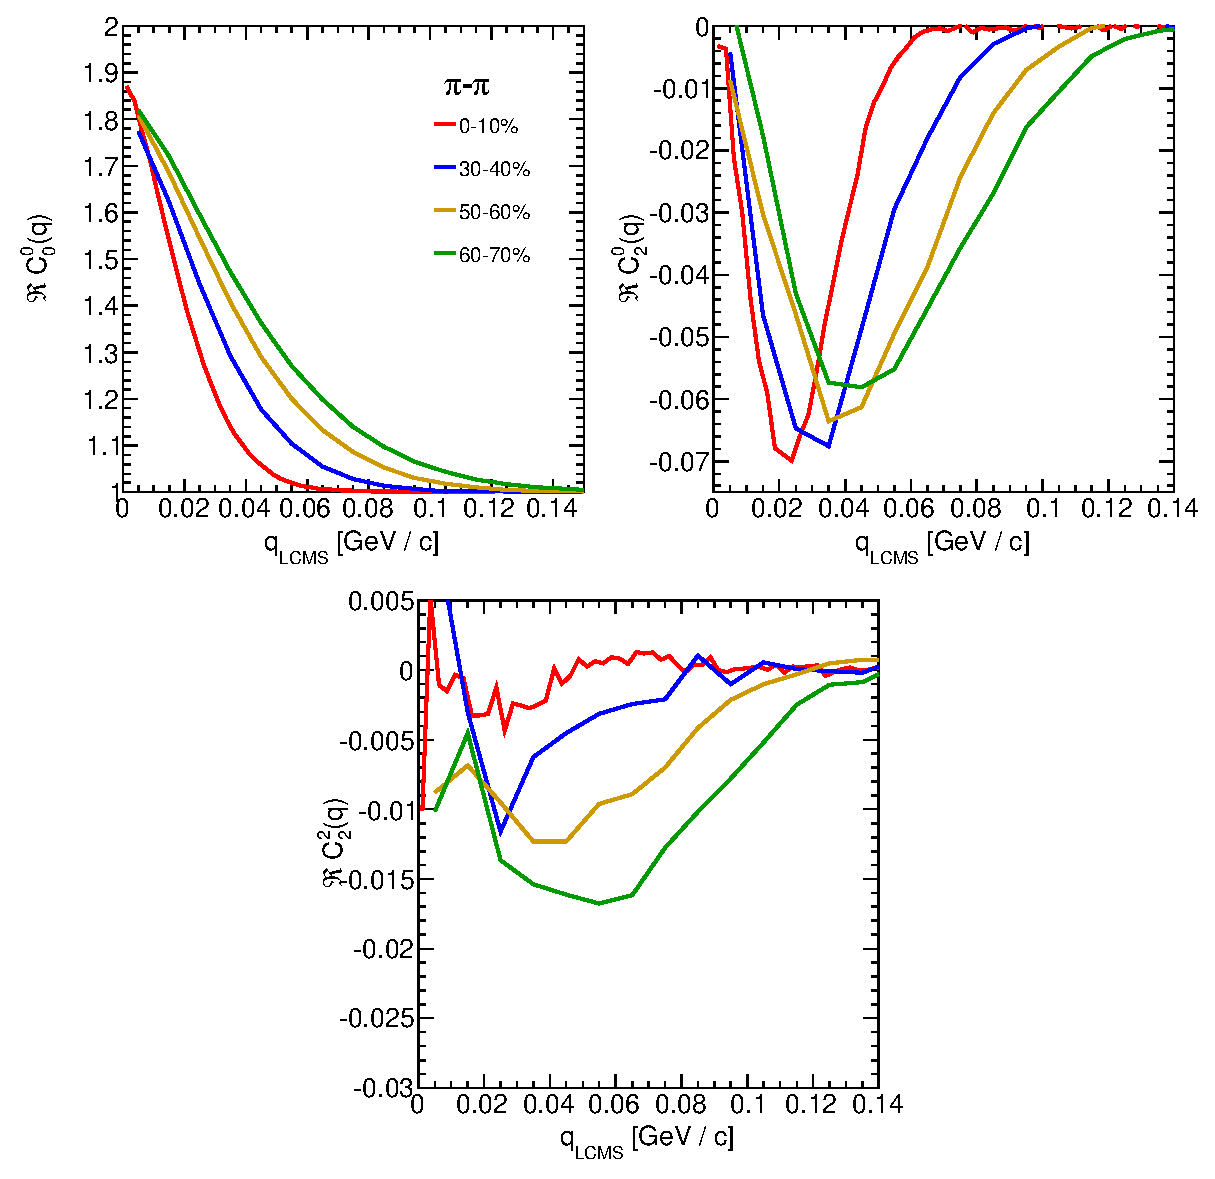
\includegraphics[width=1.0\textwidth]{results/cf3dpi}}
        \caption{Spherical harmonics coefficients of the two-pion correlation function. From the top left: $\Re C^0_0$, $\Re C^0_2$ and $\Re C^2_2$. Only few centrality bins are presented for increased readability.}
      \label{fig:cf3dpi}
      \end{figure}

      \begin{figure}[b]
        \centering
        \centerline{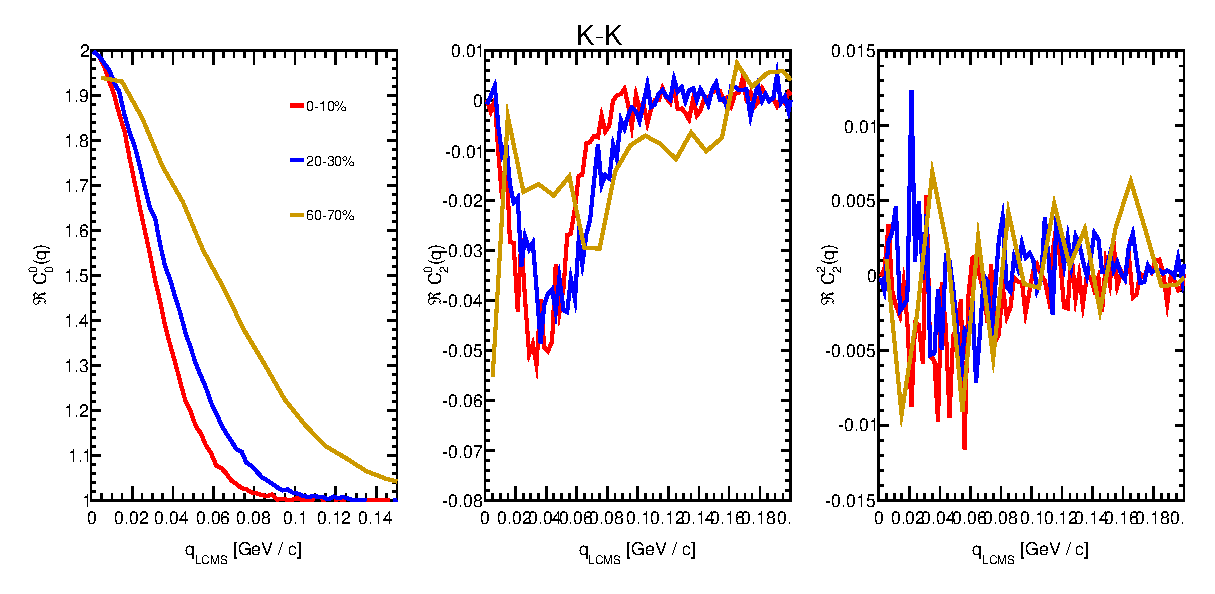
\includegraphics[width=1.0\textwidth]{results/cf3dk}}
        \caption{Spherical harmonics coefficients of the two-kaon correlation function. From the top left: $\Re C^0_0$, $\Re C^0_2$ and $\Re C^2_2$. Only few centrality bins are presented for increased readability. The $\Re C^2_2$ is noisy, but one can still notice that it differs from zero and is becoming negative.}
      \label{fig:cf3dk}
      \end{figure} 

      \begin{figure}[b]
        \centering
        \centerline{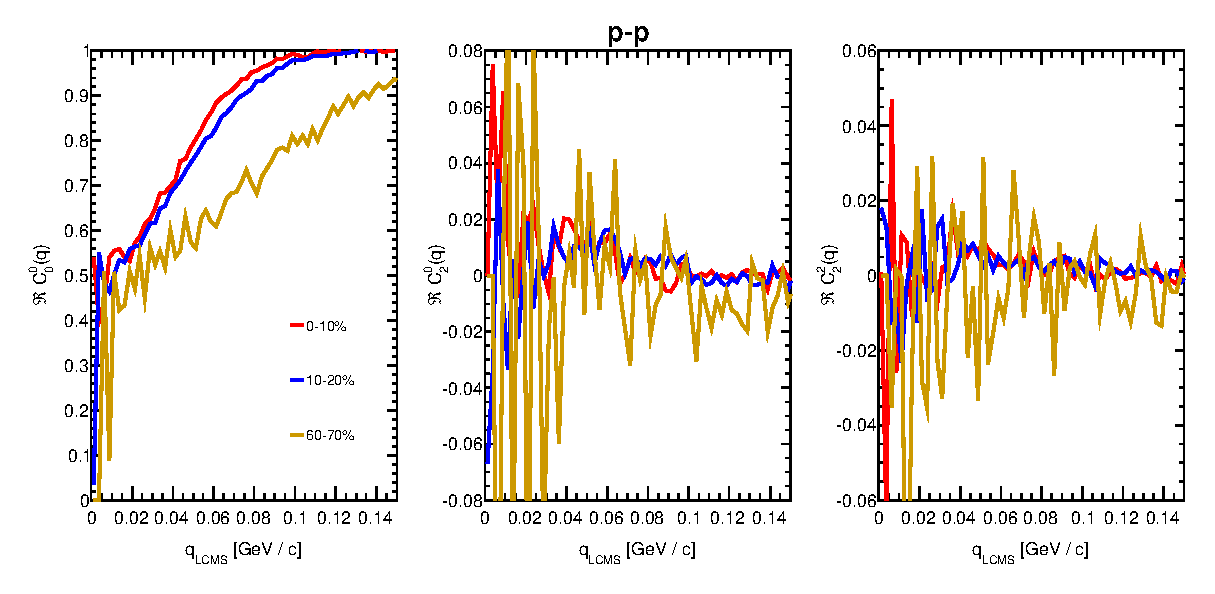
\includegraphics[width=1.0\textwidth]{results/cf3dp}}
        \caption{Spherical harmonics coefficients of the two-proton correlation function. From the top left: $\Re C^0_0$, $\Re C^0_2$ and $\Re C^2_2$. Only few centrality bins are presented for increased readability. The $\Re C^0_2$ and $\Re C^2_2$ are noisy, but one can still notice, that they differ from zero and are becoming positive.}
      \label{fig:cf3dp}
      \end{figure}

      The three-dimensional correlation function as a function of relative momentum $q_{LCMS}$ was calculated in a form of components of spherical harmonics series accordingly to the Eq.~\ref{eq:sh_decomposition}.
      In the femtoscopic analysis of identical particles, the most important information is stored in the $\Re C^0_0$, $\Re C^0_2$ and $\Re C^2_2$, hence only those components were analyzed.
      Correlation functions obtained in this procedure were calculated for the different centrality bins for the pairs of pions, kaons and protons.
      They are presented in the Fig.~\ref{fig:cf3dpi}, \ref{fig:cf3dk} and \ref{fig:cf3dp}.
      
      Coefficients for pairs of identical bosons (pions and kaons) are shown in the Fig.~\ref{fig:cf3dpi} and \ref{fig:cf3dk}.
      The wave function symmetrization (Bose-Einstein statistics) causes the increase of a correlation in the low relative momenta regime ($q_{LCMS}<0.06$~GeV/c or even $q_{LCMS}<0.12$~GeV/c for more peripheral collisions).
      It is clearly visible in the $\Re C^0_0$ component.
      The $\Re C_0^0$ resembles one-dimensional correlation function and in fact it encodes information about overall source radius.
      The second coefficient $\Re C^0_2$ differs from zero (is negative), which yields the information about the ratio $R_T / R_{long}$.
      The $\Re C^2_2$ stores the $R_{out} / R_{side}$ ratio and one can notice that is non-vanishing (is also negative).

      The correlation function for a pair of identical fermions is presented in the Fig.~\ref{fig:cf3dp}.
      An influence of wave function anti-symmetrization (Fermi-Dirac statistics) has its effect in the decrease of a correlation down to 0.5 at low relative momentum ($q_{LCMS}<0.1$~GeV/c or $q_{LCMS}<0.15$~GeV/c for more peripheral collisions), which can be observed in $\Re C^0_0$.
      The $\Re C^0_2$ and $\Re C^2_2$ coefficients differ from zero and are becoming positive.

      The common effect of the spherical harmonics form of a correlation function is the ``mirroring'' of the shape of the $\Re C^0_0$ coefficient - when correlation function increases at low $q_{LCMS}$, the $\Re C^0_2$ and $\Re C^2_2$ are becoming negative and vice versa.
      This is quite different behaviour than in the case of correlations of non-identical particles, where the $\Re C^0_2$ still behaves in the same manner, but $\Re C_2^2$ has the opposite sign to the $\Re C^0_2$~\cite{nonidfemto}.

      In all cases, the correlation function gets wider with the peripherality of a collision i.e. the correlation function for most central collisions (0-10\%) is much narrower than for the most peripheral ones (60-70\%).
      This phenomena in clearly visible the $\Re C^0_0$ coefficients.
      Other components are also affected by this effect, this is especially noticeable in the case of kaons and pions.
      For the protons, the results are noisy, hence this effect is not clearly distinguishable.

      % The quantitative analysis of the trends in the shape (described by the femtoscopic radii) of a three-dimensional correlation function is performed in the next section of this chapter.

    \FloatBarrier
    \clearpage
    %
    % ========
    \subsection{Centrality dependence of a correlation function}
    % ========
      The centrality dependence of a correlation function is especially visible in one-dimensional correlation functions.
      This effect is presented in the Fig.~\ref{fig:centr_dep} - the correlation functions for pions, kaons and protons are plotted for the same $k_T$ range but different centrality bins.
      One can notice that the width of a function is smaller in the case of most central collisions.
      Hence, the femtoscopic radii (proportional to the inverse of width) are increasing with the centrality.
      An explanation for this growth is that in the most central collisions, a size of a created system is larger than for the peripheral ones.
      \begin{figure}[h]
        \centering
        \centerline{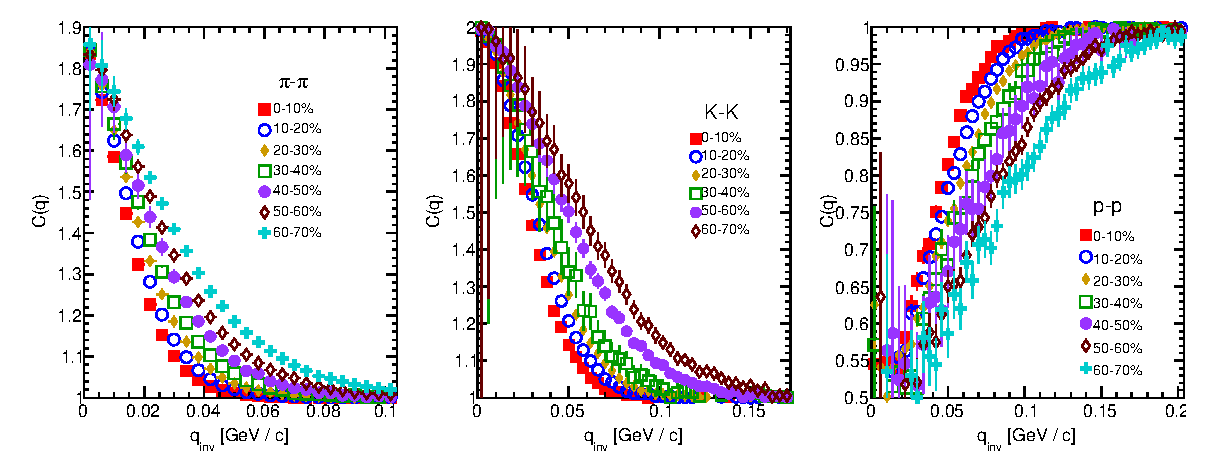
\includegraphics[width=1.0\textwidth]{results/cfvsctr}}
        \caption{One-dimensional correlation function for pions(top left), kaons (top right) and protons (bottom) for different centralities.}
      \label{fig:centr_dep}
      \end{figure}
    \FloatBarrier
    \clearpage
    %
    % ========
    \subsection{$k_T$ dependence of a correlation function}
    % ========
      In the Fig.~\ref{fig:kt_dep} there are presented one-dimensional correlation functions for pions, kaons and protons for the same centrality bin, but different $k_T$ ranges.
      One can observe in all cases of the particle types, appearance of the same trend: with the increase of the total transverse momentum of a pair, the width of a correlation function increases and the femtoscopic radius decreases.
      The plots in the Fig.~\ref{fig:kt_dep} were zoomed in to show the influence of $k_T$.

      \begin{figure}[h]
        \centering
        \centerline{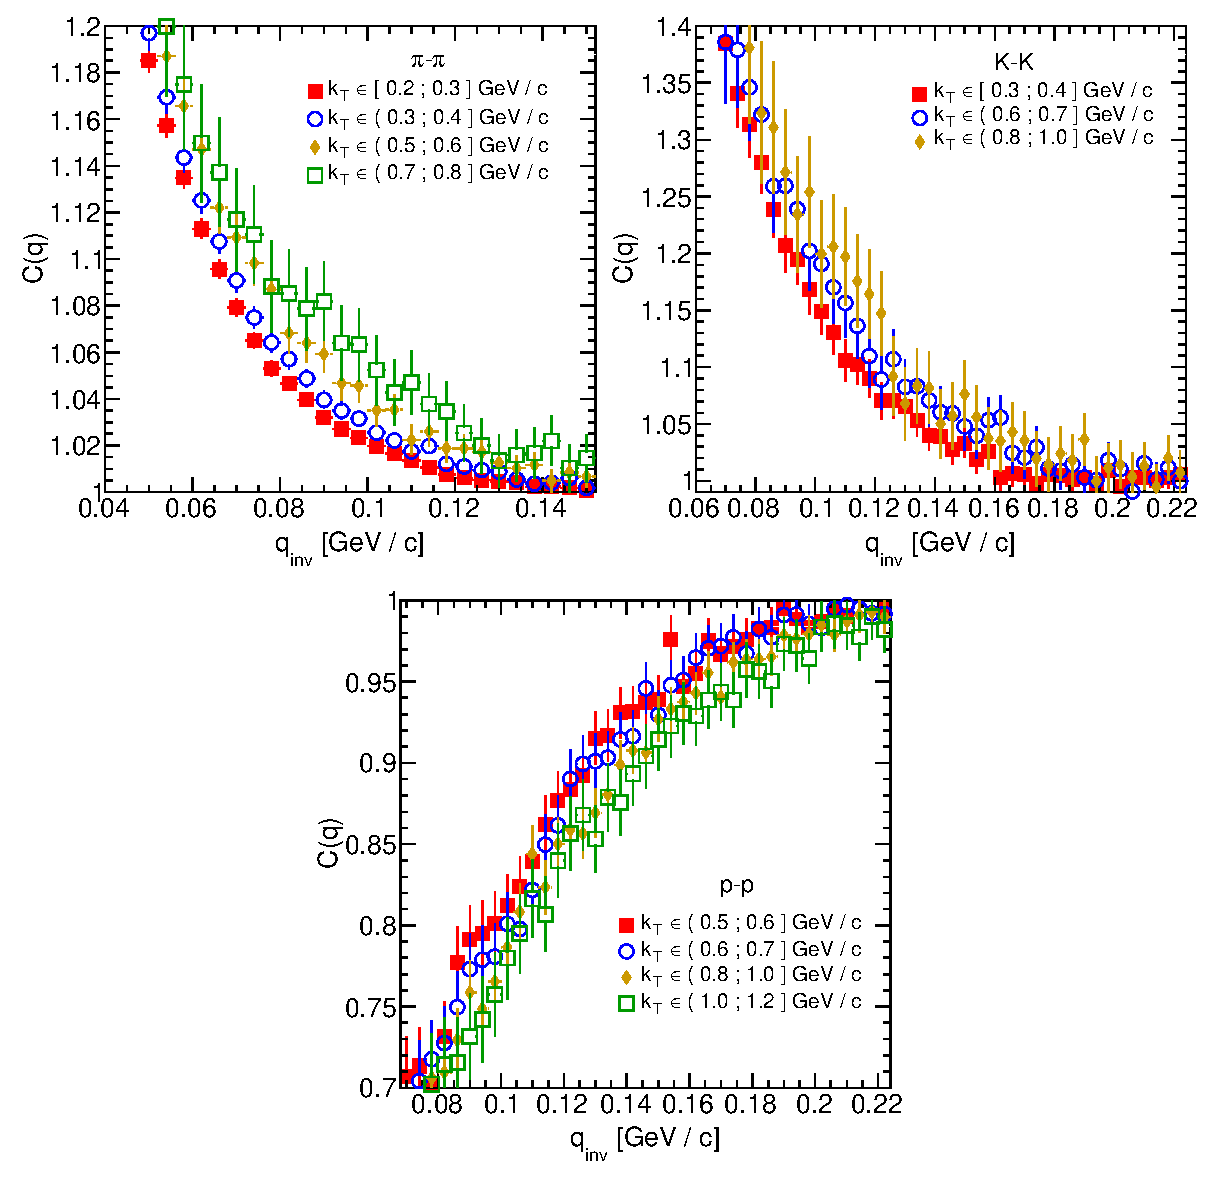
\includegraphics[width=1.0\textwidth]{results/cfvskt}}
        \caption{One-dimensional correlation functions for pions, kaons and protons, for the same centrality bin and different $k_T$ ranges. The plot was zoomed in to the region which illustrates the $k_T$ dependence in the best way. Only few of the calculated ranges are presented for better readability.}
      \label{fig:kt_dep}
      \end{figure}
    \FloatBarrier
    \clearpage
  %
  % ========
  \section{Results of the fitting procedure}
  % ========
  In order to perform a quantitative analysis of a wide range of correlation functions, the theoretical formulas were fitted to the calculated experimental-like data.
  In this procedure, the femtoscopic radii for the three-dimensional as well as one-dimensional correlation functions were extracted.
  The main goal of this analysis is a verification of a common transverse mass scaling for different particles types.
  Obtained radii are plotted as a function of a transverse mass $m_T = \sqrt{k_T^2 +m^2}$.
  To test the scaling, the following power-law was fitted to the particular radii afterwards:
  \begin{equation}
    \label{eq:power-law}
    R_x = \alpha {m_T}^{-\beta}~,
  \end{equation}
  where the $\alpha$ and $\beta$ are free parameters.
    %
    % ========
    \subsection{The three-dimensional femtoscopic radii scaling}
    % ========
      \begin{figure}[b]
        \centering
        \centerline{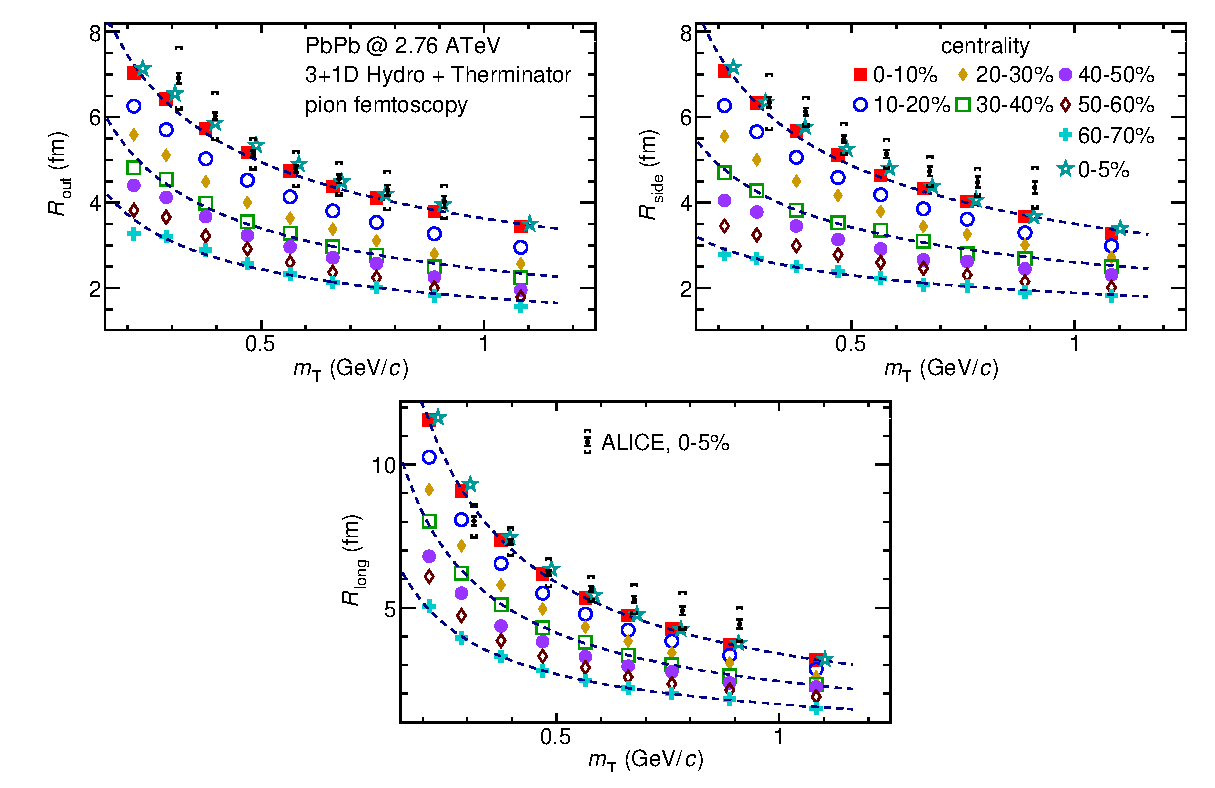
\includegraphics[width=1.05\textwidth]{results/piradii}}
        \caption{Femtoscopic radii in LCMS coming from two-pion correlation functions for all centrality bins as a function of $m_T$. The dashed lines are power-law fits. The most central collisions (0-5\%) are compared to the results from ALICE~\cite{alice_pion}. The two datasets are shifted to the right for visibility~\cite{galazyn}.}
        \label{fig:piradii}
      \end{figure}

      In the Fig.~\ref{fig:piradii} there are presented femtoscopic radii in the outward, sideward and longitudinal directions for the analysis of two-pion correlation functions in the LCMS.
      The dashed lines are fits of the power law to the data.
      One can notice, that the power law describes well data points with a 5\% accuracy.
      The $\beta$ fit parameter for the outward direction is in the order of 0.45.
      For the sideward direction, this parameter has the similar value, but it is lower for the most peripheral collisions.
      In case of the longitudinal direction, the $\beta$ has greater value, up to 0.75.
      In the Fig.~\ref{fig:piradii} there are also compared results for the top 5\% central collisions (star-shaped markers) with experimental data from ALICE~\cite{alice_pion}.
      The experimental results are consistent with the ones coming from the model predictions.
      % \begin{figure}[b]
      %   \centering
      %   \centerline{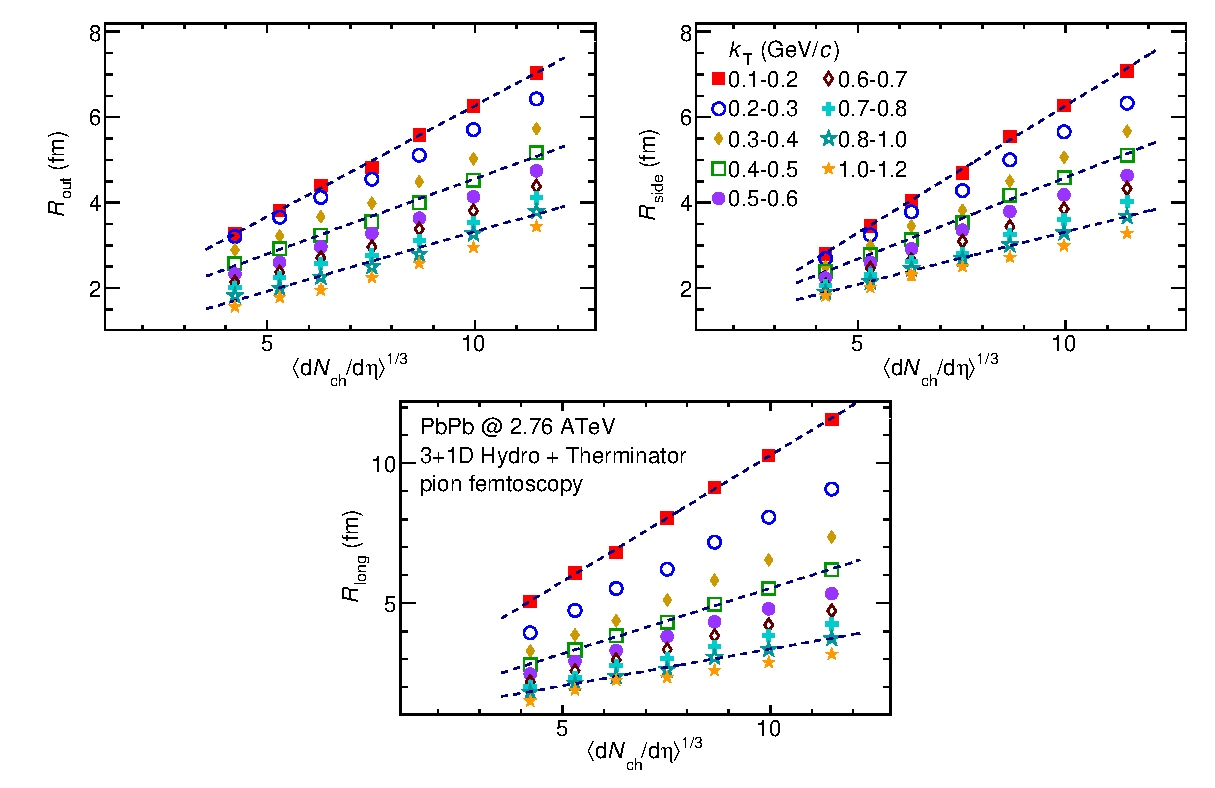
\includegraphics[width=1.05\textwidth]{results/piradii_vs_nch}}
      %   \caption{no caption~\cite{galazyn}.}
      % \label{fig:piradii}
      % \end{figure}   
      \begin{figure}[b]
        \centering
        \centerline{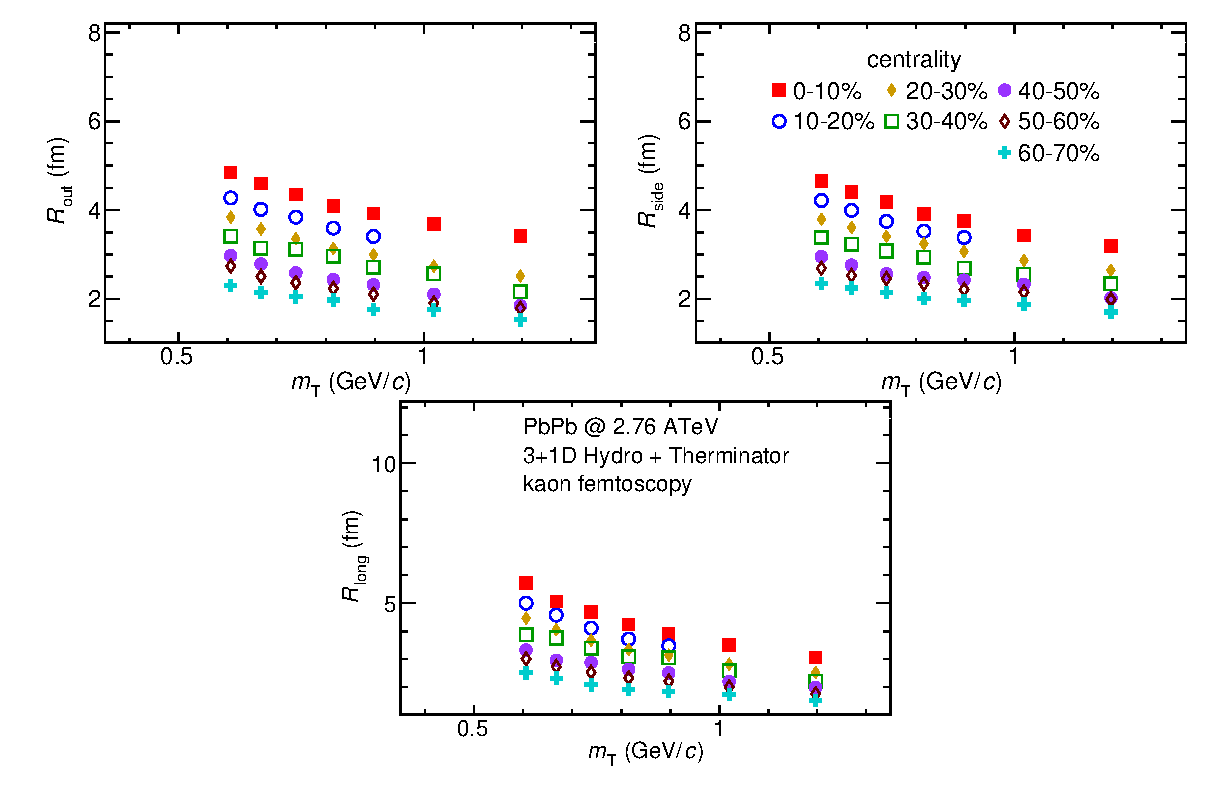
\includegraphics[width=1.05\textwidth]{results/kradii}}
        \caption{Femtoscopic radii extracted from two-kaon correlation functions for different centrality bins as a function of $m_T$.~\cite{galazyn}.}
      \label{fig:kradii}
      \end{figure}

      The Fig.~\ref{fig:kradii} presents femtoscopic radii coming from the kaon calculations.
      The $R_{out}$, $R_{side}$ and $R_{long}$ fall also with the power-law within the 5\% accuracy.
      The $\beta$ parameter was larger in case of kaons: 0.59 in outward direction, 0.54 in the sideward and 0.86 for longitudinal.

      The results for two-proton analysis are shown in the Fig.~\ref{fig:pradii}.
      The Eq.~\ref{eq:power-law} was fitted to the data and tells that the protons also follow the $m_T$ scaling within 5\% range.
      The $\beta$ parameter values were even bigger for the outward ( 0.58 ), sideward ( 0.61 ) and longitudinal ( 1.09 ) directions than for the other particle types. 

      \begin{figure}[b]
        \centering
        \centerline{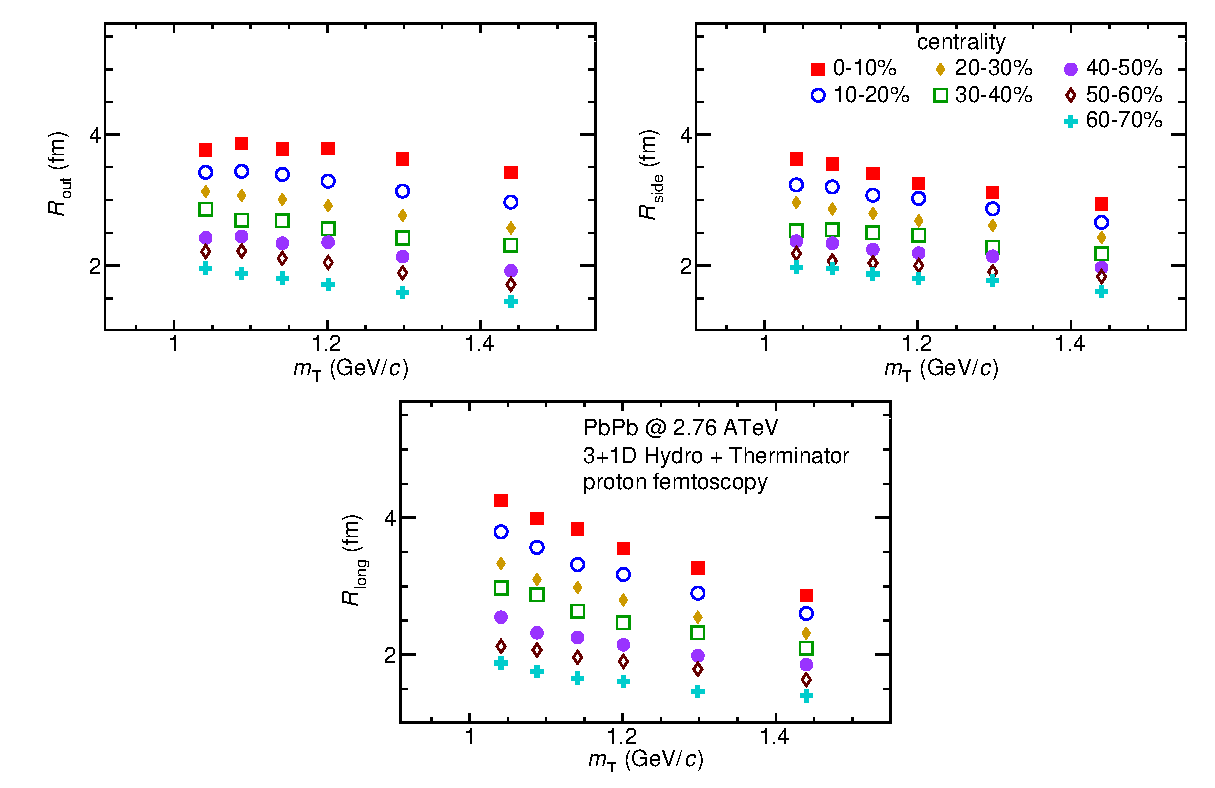
\includegraphics[width=1.05\textwidth]{results/pradii}}
        \caption{Femtoscopic radii extracted from two-proton correlation functions for different centrality bins as a function of $m_T$.~\cite{galazyn}.}
      \label{fig:pradii}
      \end{figure}

      \begin{figure}[b]
        \centering
        \centerline{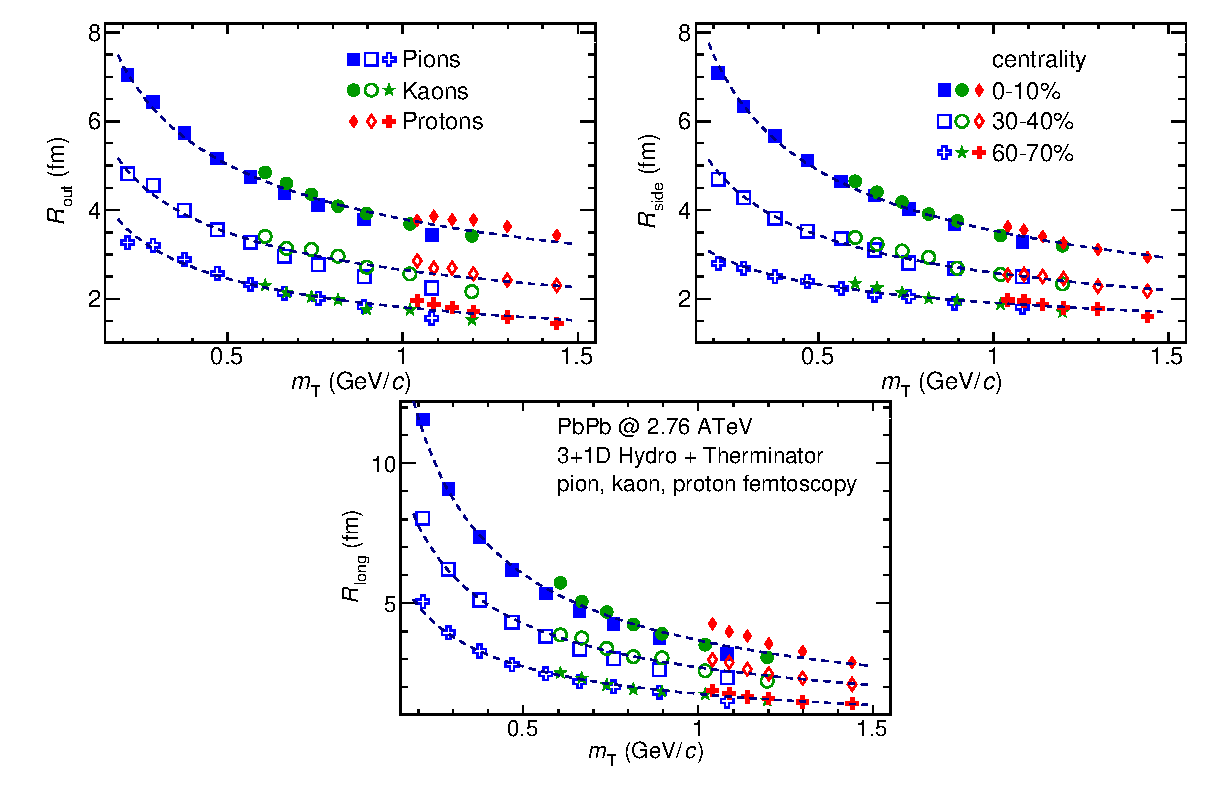
\includegraphics[width=1.05\textwidth]{results/allradii_lcms}}
        \caption{The results from the calculations for the pions, kaons and protons in for the three centralities presented on the common plot. One can notice that radii for particular centralities and different particle types follow the common power-law scaling.~\cite{galazyn}.}
      \label{fig:allradii}
      \end{figure}    

      The Fig.~\ref{fig:allradii} presents results for the pions, kaons and protons together as a function of $m_T$.
      Considering differences in the $\beta$ value for the fits for different particles, one can suspect that there is no common scaling between different kinds of particles.
      However, when all of the results shown on the same plot, they are aligning on the common curve and the scaling is well preserved.
      The scaling accuracy is 3\%, 5\% and 4\% for the 0-10\%, 20-30\% and 60-70\% for the outward direction.
      For the sideward radii the scaling is better, with average deviations 2\%, 2\% and 3\% respectively.
      In case of longitudinal direction the accuracy is 6\%, 5\% and 3\% for the three centralities.
      The $\beta$ parameter for the outward direction is close to the 0.42 in all cases.
      For the sideward direction it varies from 0.28 to 0.47 and is bigger for more central collisions.
      Regarding longitudinal radii, the exponent is bigger than the other two: $\beta \in [0.62 ; 0.72]$~.
      Considering all results, the plotted radii are following the common power-law scaling within the 5\% accuracy for all directions, centralities and particle types.
      \FloatBarrier
      %
      % ========
      \subsection{Scaling of one-dimensional radii}
      % ========
      To the one-dimensional correlation function, the corresponding function in the PRF given by the Eq.~\ref{eq:cf_1d} was fitted.
      The results from those fits are presented in the upper left plot in the Fig.~\ref{fig:scaling_test}.
      One immediately notices, that there is no common scaling of $R_{inv}$ for different kind of particles.
      In the Fig.~\ref{fig:allradii} the radii in the outward direction for the pions, kaons and protons for the same $m_T$ are similar.
      However, when one performs a transition from the LCMS to the PRF, the $R_{out}$ radius grows:
      \begin{equation}
        {R_{out}}^{*} = \gamma_T R_{out}~,
      \end{equation}
      where $\gamma_T = m_T / m$.
      For the lighter particles, the $\gamma_T$ is much larger, hence the bigger growth of the $R_{out}$ and the overall radius.
      This is visible in the Fig.~\ref{fig:scaling_test} (top left), where the radii in the PRF for the lighter particles are bigger than for the heavier ones in case of the same $m_T$ range.

      In the Fig.~\ref{fig:allradii} there is visible scaling in the outward, sideward and longitudinal direction.
      Hence one can expect an appearance of such scaling in a direction-averaged radius calculated in the LCMS.
      This radius is presented in the Fig.~\ref{fig:scaling_test} (bottom) and indeed the $R_{LCMS}$ exhibits power-law scaling with the $m_T$.

      \begin{figure}[b]
        \centering
        \centerline{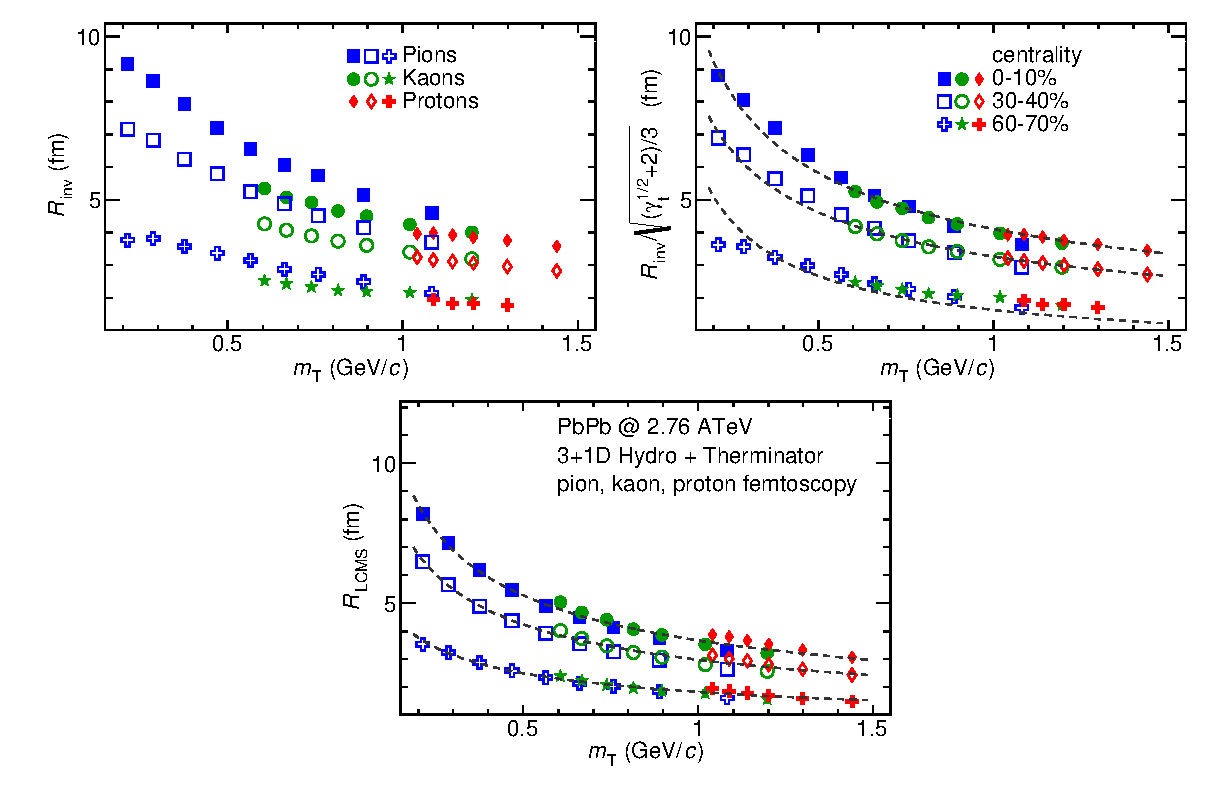
\includegraphics[width=1.05\textwidth]{results/scaling_test}}
        \caption{Top left: one-dimensional radius for pions, kaons and protons calculated in the PRF. Top right: the $R_{inv}$ scaled by the proposed factor. Bottom: averaged one-dimensional radius in the LCMS for pions, kaons and protons. Only three centrality bins are shown for the better readability~\cite{galazyn}.}
      \label{fig:scaling_test}
      \end{figure}

      One can try to account the effect of an increase of the radii in the outward direction by using the appropriate scaling factor.
      In the Fig.~\ref{fig:scaling_test} (top right) there are femtoscopic radii in the LCMS divided by the proposed scaling factor:
      \begin{equation}
        f = \sqrt{ \left. \left( \sqrt{\gamma_T} + 2 \right) \middle/ 3 \right. }~.
      \end{equation}
      The radii for pions, kaons and protons in the PRF after the division by $f$ are following the power-law with the accuracy of 10\%.

      % \begin{figure}[b]
      %   \centering
      %   \centerline{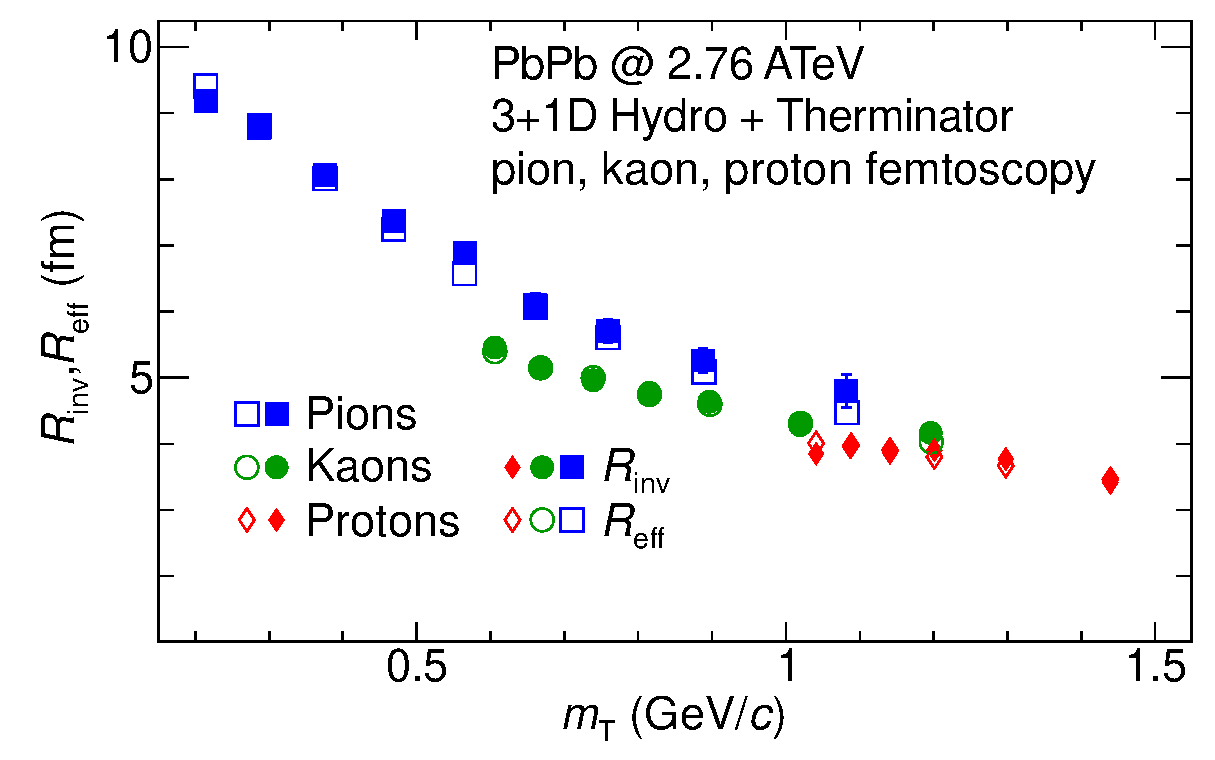
\includegraphics[width=0.55\textwidth]{results/rinvreff}}
      %   \caption{no caption~\cite{galazyn}.}
      % \label{fig:rinveff}
      % \end{figure}


      \FloatBarrier
  %
  % ========
  \section{Discussion of the results}
  % ========
    The femtoscopic radii obtained from the three-dimensional correlation function fitting exhibit the $m_T$ dependence described by the power law (Eq.~\ref{eq:power-law}).
    This scaling is preserved quite well with accuracy <10\%.
    Observation of such scaling in a femtoscopic radii is a strong signal of appearance of a collective behaviour of a particle-emitting source created in the collision.
    The data used in the analysis was coming from the hydrodynamic model, hence one can indeed expect the appearance of this scaling.
    However, the results for pion femtoscopy from the ALICE at LHC are consistent with the data from analysis performed in this thesis (Fig.~\ref{fig:piradii}).
    This is a confirmation of an applicability of hydrodynamic models in a description of an evolution of a quark-gluon plasma.

    The $\beta$ parameter calculated in the fitting of the power-law to the femtoscopic radii is in the order of 0.5 in case of the radii in the transverse plane.
    This value is consistent with the hydrodynamic predictions.
    In case of longitudinal radii, the exponent is bigger (greater than 0.7), which is an indication of a strong transversal expansion in the system~\cite{akkelin_sinyukov}.

    A scaling described above is visible in the LCMS, however due to limited statistics, analysis in this reference frame is not always possible.
    In such case one performs calculations in the PRF.
    The $m_T$ scaling in the PRF is not observed - this has the trivial kinematic origin.
    A transition from the PRF to LCMS causes growth of the radius in the outward direction and the common power-law scaling for different particles breaks due to differences in the $\gamma_T (m_T)$ for different particle types.
    However one can try to deal with the radius growth and restore the scaling by multiplying the radii $R_{inv}$ by an approximate factor $\sqrt{ \left. \left( \sqrt{\gamma_T} + 2 \right) \middle/ 3 \right. }$.
    The scaled $R_{inv}$ are following the power-law and could be used as a verification of hydrodynamic behaviour in the investigated particle source.

    The hadronic evolution and freeze-out in the \verb|THERMINATOR| is followed by the resonance propagation and decay phase.
    A good accuracy of a scaling with the power-law indicated that the inclusion of the resonances does not break the $m_T$ scaling.
    However, recent calculations including also hadron rescattering phase indicate that the scaling between pions and kaons is broken at the LHC~\cite{sinyukov_kaon}.
